%----------------------------------------------------------------------------------------
%	PACKAGES AND THEMES
%----------------------------------------------------------------------------------------
% handout option removes the pauses
\documentclass[aspectratio=169,xcolor=dvipsnames]{beamer}
\usetheme{SimplePlus}

\usepackage{hyperref}
\usepackage{graphicx} % Allows including images
\usepackage{booktabs} % Allows the use of \toprule, \midrule and \bottomrule in tables
\usepackage{listing}  % see style.sty file

%----------------------------------------------------------------------------------------
%	TITLE PAGE
%----------------------------------------------------------------------------------------

\title{Direct Style (for asynchronous programming) in Scala}
\subtitle{The Scala \texttt{gears} library}

\author{Luca Tassinari}

% \institute[NTU] % Your institution as it will appear on the bottom of every slide, may be shorthand to save space
%{
%    Department of Computer Science and Information Engineering \\
%    National Taiwan University % Your institution for the title page
%}
\date{\today} % Date, can be changed to a custom date

%----------------------------------------------------------------------------------------
%	PRESENTATION SLIDES
%----------------------------------------------------------------------------------------

\begin{document}

\begin{frame}
    % Print the title page as the first slide
    \titlepage
\end{frame}

\begin{frame}{Overview}
    % Throughout your presentation, if you choose to use \section{} and \subsection{} commands, these will automatically be printed on this slide as an overview of your presentation
    \tableofcontents
\end{frame}

%----------------------------------------------------------------------------------------
\section{Context}
%----------------------------------------------------------------------------------------

\begin{frame}{From Monads to Capabilities}
    \begin{itemize}
        \item Most of the times when we say \emph{effect} we mean \emph{monads}
        \item Monads do have cons:
        \begin{itemize}
            \item awkward to integrate with regular control structures
            \item composing them is complex
            \item syntactic and pedagogical overhead
        \end{itemize}
    \end{itemize}

    \begin{block}{}
        Ongoing research project: instead of pushing effects and resources into frameworks, upgrade the type system to track them directly in the program $\Rightarrow$ \textbf{CAPabilities for RESources and Effects (CAPRESE)} @ Programming Methods Laboratory EPFL \cite{capabilities}.
    \end{block}

    Idea:
    \begin{itemize}
        \item to have
        an effect you need the related \textbf{capability};
        \item a \textit{capability} is just a value passed to the function (usually implicitly) that needs to perform the effect the capability enables.
    \end{itemize}
\end{frame}

%----------------------------------------------------------------------------------------

\begin{frame}
    To model a function that could throw an exception
    \footnote{\tiny
        These examples are experimental features of Scala 3 and require to be compiled with \texttt{-experimental} flag or marked as \texttt{@experimental}.
    }:
    \lstinputlisting[language=scala]{listings/CanThrow1.scala}
    
    Under the hood, the compiler generates the \texttt{CanThrow} capability:
    \lstinputlisting[language=scala]{listings/CanThrow2.scala}
\end{frame}

%----------------------------------------------------------------------------------------

\begin{frame}
    \begin{itemize}
        \item<1-> If the capability is not provided: compilation error!
        \lstinputlisting[language=scala]{listings/CanThrow3.scala}
        \item<2-> We can pass to a higher-order function a function encapsulating an effect without changing its signature!
        \lstinputlisting[language=scala]{listings/CanThrow4.scala}
    \end{itemize}
\end{frame}

%----------------------------------------------------------------------------------------

\begin{frame}{Algebraic effects}
    Not just exceptions...
    \begin{block}{}
        Algebraic Effects $\equiv$ exceptions + \texttt{resume} operation \cite{can-throw}
    \end{block}
    The \texttt{resume} operation allows to resume the computation from the point where the effect was raised, after having \textbf{handled} it
    \lstinputlisting[language=scala]{listings/AsyncSupport.scala}
\end{frame}

%----------------------------------------------------------------------------------------

\begin{frame}{Generator effect \cite{scalar-gears}}
    Pyhton-like generator to get all the leafs of a tree:

    \lstinputlisting[language=scala]{listings/TreeGenerator.scala}
\end{frame}

%----------------------------------------------------------------------------------------

\begin{frame}
    \lstinputlisting[language=scala]{listings/Generator.scala}   
\end{frame}

%----------------------------------------------------------------------------------------

\begin{frame}
    \begin{block}{Takeaways}
        \begin{itemize}
            \item Capabilities + delimited continuations enables Algebraic effects
            \begin{itemize}
                \item With algebraic effects, instead of focusing on how to concatenate the effects, we focus on their definition and interpretation (i.e. how to handle them)
            \end{itemize}
            \item Thanks to continuations is possible to design a library for asynchronous computation exploiting \textbf{direct style}, i.e. imperative-like code.
        \end{itemize}
    \end{block}
\end{frame}

%--------------------------------------------------------------------------------

\begin{frame}{Boundary \& Break \cite{scalar-gears}}
    \begin{itemize}
        \item boundary \& break is a mechanism providing a cleaner alternative to non-local returns
        \lstinputlisting[language=scala]{listings/BBreak.scala}
        \item it is important to implement the \texttt{resume mechanism}
        \item can be useful for error handling and inner loops where we need a short exit path
    \end{itemize}
\end{frame}

%----------------------------------------------------------------------------------------

\begin{frame}
    Leveraging boundary \& break it's possible to implement data types to handle errors (usage examples will be shown later):
    \lstinputlisting[language=scala]{listings/Either.scala}   
\end{frame}

%----------------------------------------------------------------------------------------
\section{Scala \texttt{gears}}
%----------------------------------------------------------------------------------------

\begin{frame}{Suspension effect, Scala \texttt{gears} \cite{gears}}
    \begin{itemize}
        \item New \emph{strawman} library for asynchronous computation using \textbf{direct style}.
        \item Designed to be \emph{cross platform}: implements the suspension interface leveraging Virtual Threads (on the JVM) and Scala Native delimited continuations (on native).
    \end{itemize}
\end{frame}

%--------------------------------------------------------------------------------

\begin{frame}
    \begin{block}{Main abstractions}
        \begin{columns}[c,onlytextwidth]
            \column{.6\textwidth}
            \begin{enumerate}
                \item \texttt{Async} context is \textbf{"a capability that allows a computation to suspend while waiting for the result of an async source"}
                \lstinputlisting[language=scala]{listings/Gears-1.scala}
                \begin{itemize}
                    \item every async context has a completion group tracking all computations in a tree structure, enabling \textbf{structured concurrency}
                    \item \texttt{Async.blocking} creates an \texttt{Async} context blocking the running thread for suspension (usually placed inside the \texttt{main})
                    \lstinputlisting[language=scala]{listings/Gears-2.scala}
                \end{itemize}
            \end{enumerate}
            \column{.35\textwidth}
            \begin{figure}
                \centering
                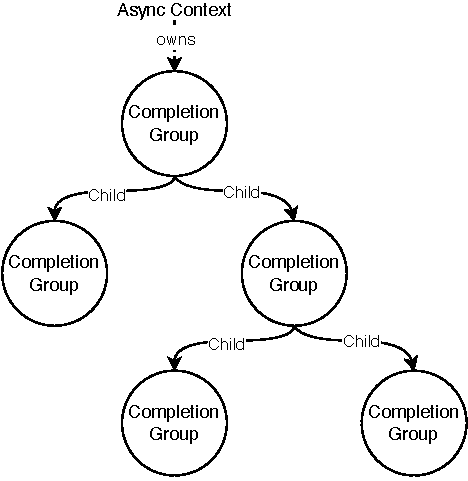
\includegraphics[width=\textwidth]{./images/structured-concurrency.pdf}
            \end{figure}
        \end{columns}
    \end{block}
\end{frame}

%--------------------------------------------------------------------------------

\begin{frame}
    \begin{block}{}
        \begin{enumerate}
            \setcounter{enumi}{1}
            \item \texttt{Async.Source} model an asynchronous source of data that can be \textbf{polled} or \textbf{awaited} by suspending the computation, as well as composed using combinator functions.
            \item \texttt{Futures} are the primary (in fact, the only) active elements \textbf{encapsulating a control flow} that, eventually, will deliver a result (either a computed or a failure value that contains an exception)
            \begin{itemize}
                \item To spawn \texttt{Future}s, the \texttt{Spawn} capability is needed. It is usually provided by the \texttt{Async.group} function.
                \lstinputlisting[language=scala]{listings/Gears-3.scala}
                \item \texttt{Tasks} represent delayed \texttt{Futures} (to make them \textit{referential transparent}), essentially wrapping a \texttt{() => Future[T]}.
            \end{itemize}
        \end{enumerate}
    \end{block}
\end{frame}

%--------------------------------------------------------------------------------

\begin{frame}
    \begin{example}[1]
        A service that allows storing in repository posts, performing checks on the content and author before the actual storage.
    \end{example}

    Desired behavior:
    \begin{itemize}
        \item the two checks can be spawned and run in parallel;
        \item whenever one of the two fails, the other gets canceled!
    \end{itemize}
\end{frame}

%--------------------------------------------------------------------------------

% \begin{frame}
%     \lstinputlisting[language=scala]{listings/PostServiceCurrent.scala}
% \end{frame}

%--------------------------------------------------------------------------------

\begin{frame}
    \lstinputlisting[language=scala]{listings/PostServiceDirect.scala}
    \fontsize{8}{10}
    \begin{itemize}
        \item \texttt{Async.group} creates a new completion group guaranteeing that all the computations spawned within it are terminated upon the completion of the group;
        \item \texttt{zip} operator allows combining the results of two \texttt{Future}s in a pair if both succeed, or fail with the first error encountered. Combined with \texttt{Async.group} the failure of one of the two determines the cancellation of the entire group.
    \end{itemize}
\end{frame}

%--------------------------------------------------------------------------------

\begin{frame}
    \begin{columns}[c,onlytextwidth] % The "t" option specifies top vertical alignment
        \column{.35\textwidth}
        \begin{block}{Producer-Consumer pattern}
        The last abstraction: \textbf{Channels}. They represent the primitive communication and coordination means to exchange Future results.
        \end{block}
        %------------------------------------------------
        \column{.6\textwidth} 
        \begin{figure}
            \centering
            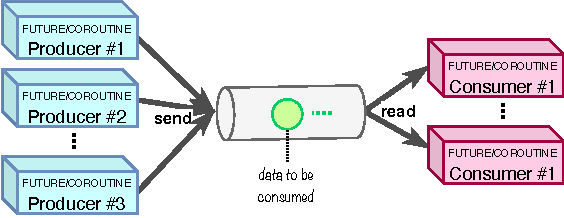
\includegraphics[width=\textwidth]{./images/channels.pdf}
        \end{figure}
    \end{columns}
    \vspace*{1em}
    \begin{itemize}
        \item Multiple producers and consumers can be "attached" to the same channel;
        \item Consumers compete with each other for sent values;
        \item Once the element is handled, it is immediately removed from the channel;
        \item \texttt{send} and \texttt{read} operations to channels are fair w.r.t. the order of their invocations from multiple process.
    \end{itemize}
\end{frame}

%--------------------------------------------------------------------------------

\begin{frame}  
    % \begin{figure}
    %     \centering
    %     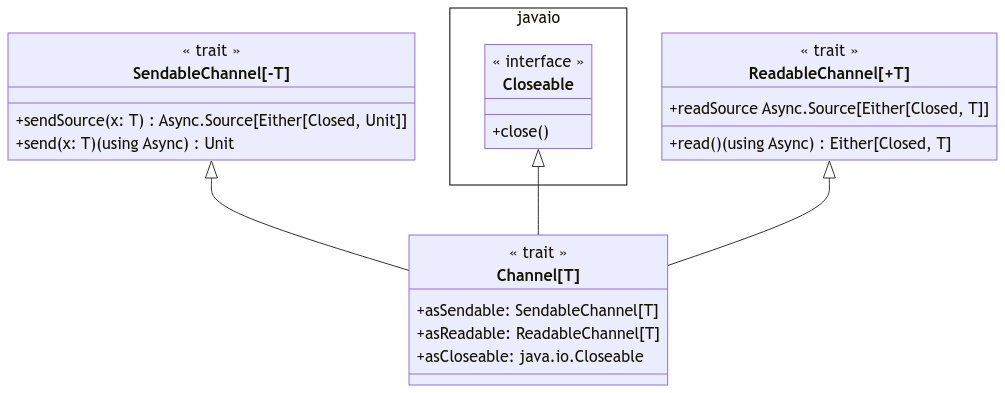
\includegraphics[width=0.9\textwidth]{./images/channels-uml.png}
    % \end{figure}
    \begin{itemize}
        \item Synchronous Channels: links a read request to a send within a rendezvous
        \begin{itemize}
            \item \texttt{send} (\texttt{read}) suspend the process until a consumer \texttt{read} (\texttt{send}) the value
        \end{itemize}
        \item Buffered Channels: a version of a channel with an internal buffer of fixed size
        \begin{itemize}
            \item \texttt{send} suspend the process if the channel is full;
            \item \texttt{read} suspend if the channel is empty, waiting for a new value.
        \end{itemize}
        \item Unbounded Channels: a version of a channel with an unbounded buffer
        \begin{itemize}
            \item if the programs run out of memory you can get an out-of-memory exception!
        \end{itemize}
    \end{itemize}
\end{frame}

%--------------------------------------------------------------------------------

\begin{frame}
    \begin{columns}[c,onlytextwidth] % The "t" option specifies top vertical alignment
        \column{.4\textwidth}
        \begin{example}[2]
            We want to realize a little asynchronous library allowing clients to collect the common statistics about repositories (issues, stars, last release) and contributors of a given GitHub organization.
        \end{example}
        \begin{itemize}
            \item Start the computation (interaction with GitHub API is required)
            \item Cancellation of the computation
        \end{itemize}
        %
        \column{.65\textwidth}
        \begin{figure}
            \centering
            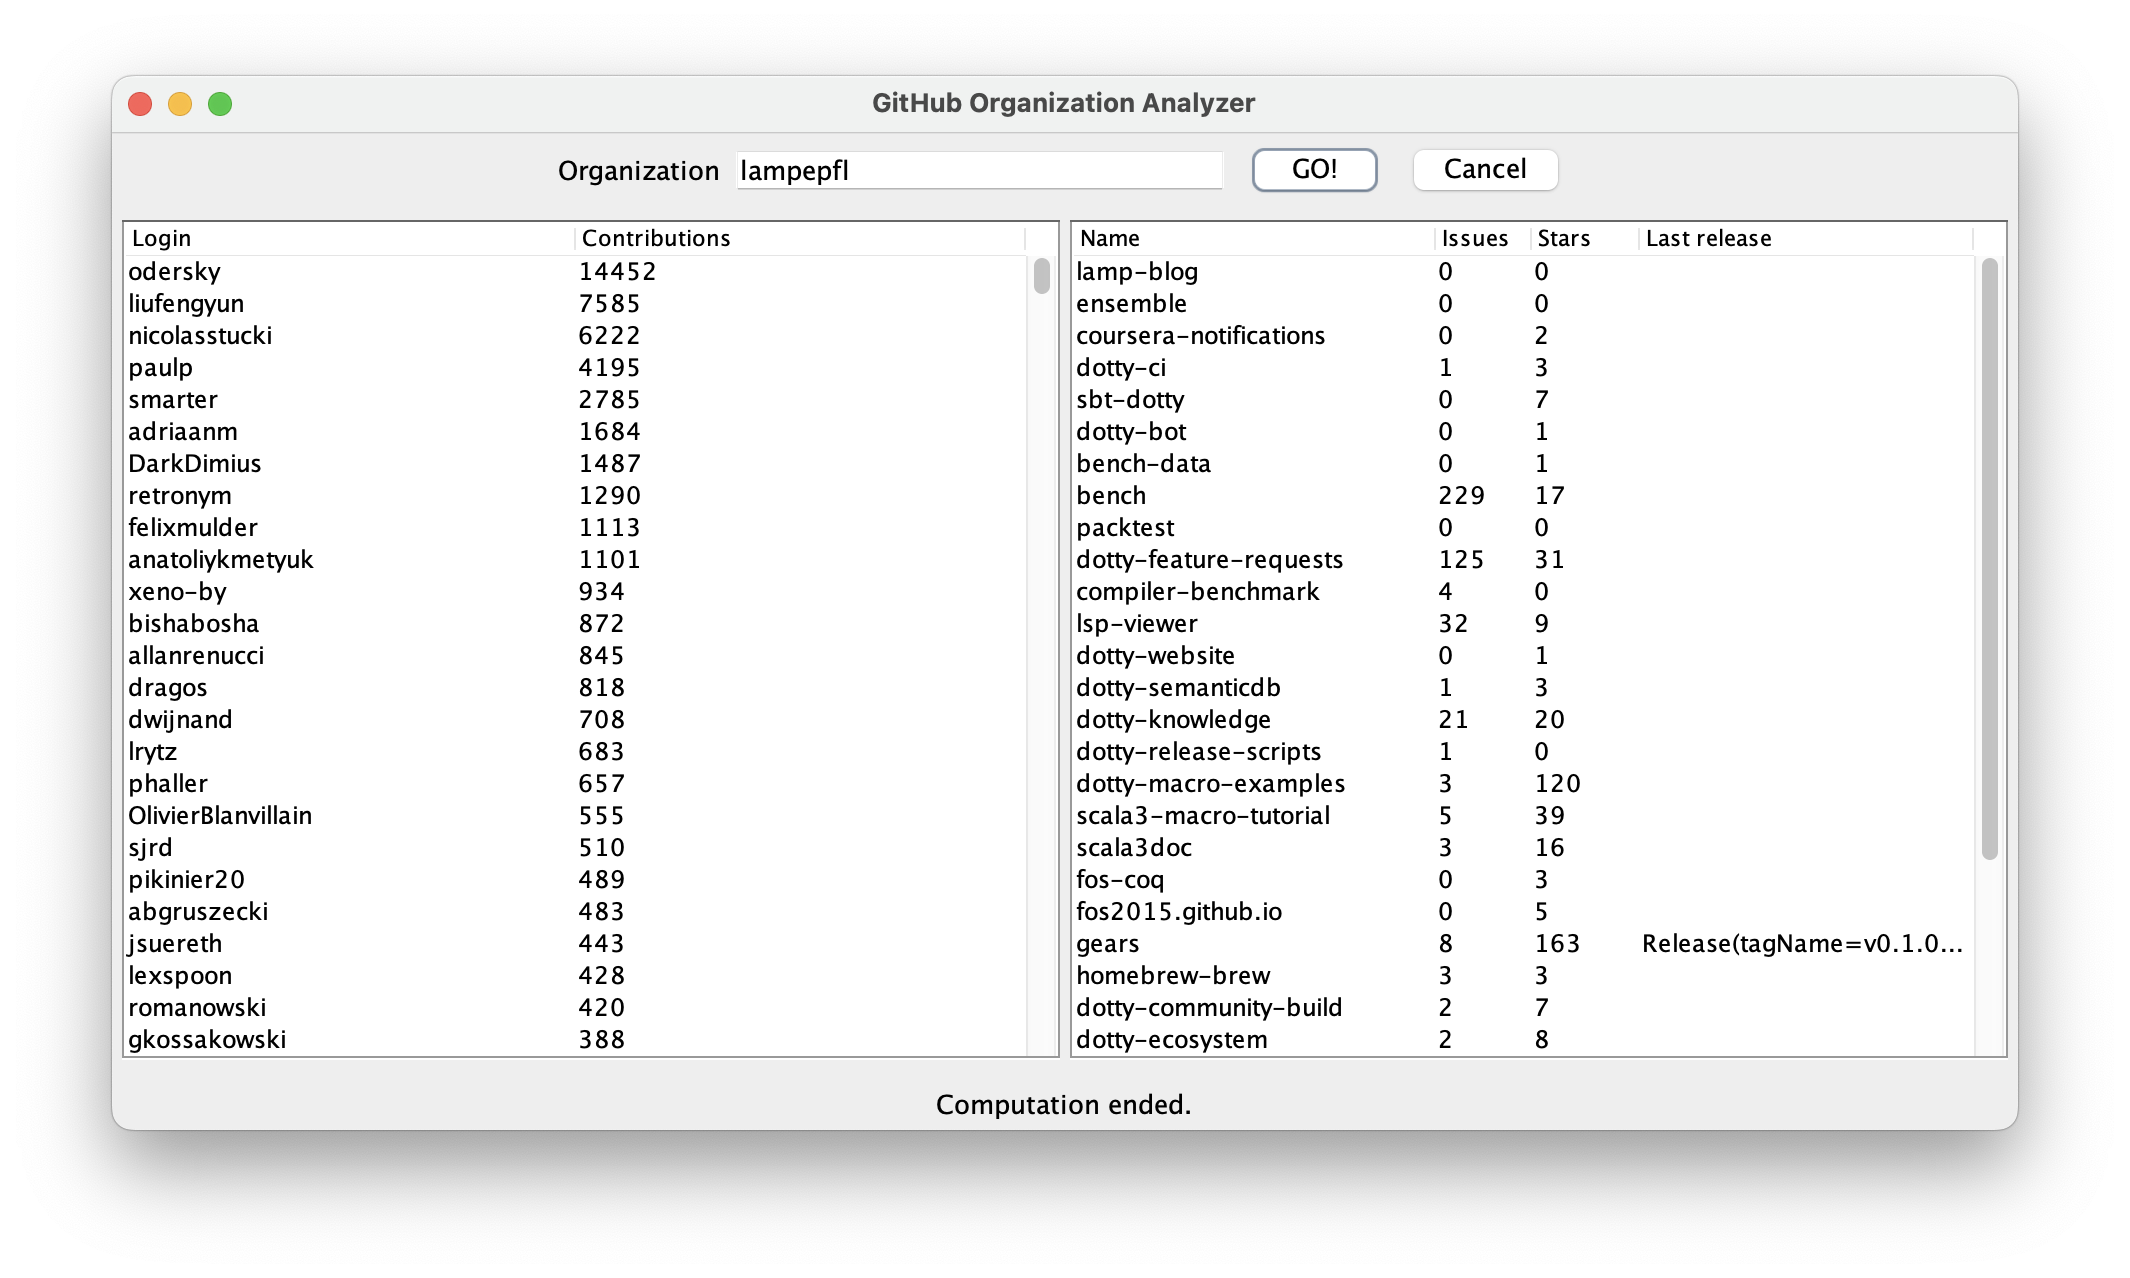
\includegraphics[width=\textwidth]{./images/analyzer-e2e.png}
        \end{figure}
    \end{columns}
\end{frame}

%--------------------------------------------------------------------------------

\begin{frame}{"Concurrency has to be explicit!"}
    The interface of the library provides a suspending method: if the client wants to perform this operation asynchronously, it has to opt in explicitly (using a \texttt{Future}).
    \lstinputlisting[language=scala]{listings/Analyzer.scala}
\end{frame}

%--------------------------------------------------------------------------------

\begin{frame}
    \lstinputlisting[language=scala]{listings/BasicAnalyzer.scala}
    \footnotesize
    \begin{enumerate}
        \item we get all the repositories of the requested organization
        \item for each of them, the contributors and the last release are retrieved concurrently, starting a \texttt{Future}
        \item \texttt{Future} results are gathered within a \texttt{Collector}, which allows a list of \texttt{Future}s to be collected in a channel, arriving as they finish.
        \item results are read from the channel as they come, calling the \texttt{updateResult} reaction function.
        \item overall results are returned to the client.
    \end{enumerate}
\end{frame}

%--------------------------------------------------------------------------------

\begin{frame}
    \begin{alertblock}{Problem 1}
        \lstinputlisting[language=scala]{listings/Problem1.scala}
        \small
        GitHub API implements pagination: if the organization has lots of repositories, the client has to deal with multiple pages of results, but the analysis can start as soon as the first page is retrieved.
    \end{alertblock}
    %
    \pause
    %
    \small$\Rightarrow$ instead of returning a \texttt{Seq[repository]} we return a \texttt{Channel[Repository]}
    %
    \pause
    %
    \begin{alertblock}{Problem 2}
        \small
        Currently, channels are closable, but once closed the consumer cannot finish reading sent values. How to notify no more results are sent?
    \end{alertblock}
    %
    \pause
    %
    \small$\Rightarrow$ \texttt{TerminableChannel}s are needed.
    \lstinputlisting[language=scala]{listings/Problem2.scala}
\end{frame}

%--------------------------------------------------------------------------------

\begin{frame}
    \lstinputlisting[language=scala]{listings/TerminableChannel.scala}
\end{frame}

%--------------------------------------------------------------------------------

\begin{frame}
    \lstinputlisting[language=scala]{listings/TerminableChannelCompanion.scala}
\end{frame}

%--------------------------------------------------------------------------------

\begin{frame}
    \small
    On top of \texttt{TerminableChannel}s is possible to implement useful methods, like \texttt{foreach} and \texttt{toSeq}:
    \lstinputlisting[language=scala]{listings/TerminableChannelOps.scala}
\end{frame}

%--------------------------------------------------------------------------------

\begin{frame}
    \lstinputlisting[language=scala]{listings/IncrementalAnalyzer.scala}
    \footnotesize
    \begin{enumerate}
        \item iterate over all the repositories sent over the channel as soon as they are retrieved by the service;
        \item we start the analysis in a separate Future: the analysis is spawned as soon as a repository is fetched by the channel, preventing starting the analysis of the next repository only when the previous one is finished;
        \item since analysis are started concurrently the \texttt{updateResult} must be called safely;
        \item we wait for the completion of all the started Futures.
    \end{enumerate}
\end{frame}

%--------------------------------------------------------------------------------

\begin{frame}
    Cons of the current implementation:
\end{frame}

%--------------------------------------------------------------------------------

\begin{frame}
    \begin{block}{Kotlin-inspired \texttt{Flow}s}
        They are very similar to cold observable in reactive programming, and they are the perfect fit for functions that need to return a \textbf{stream of asynchronously computed values}.
    \end{block}
    \lstinputlisting[language=scala]{listings/ShowcasingFlows.scala}
\end{frame}

%--------------------------------------------------------------------------------

\begin{frame}
    \begin{columns}
        \column{.45\textwidth}
        \lstinputlisting[language=scala]{listings/ShowcasingFlows2.scala}

        \lstinputlisting[language=scala]{listings/ShowcasingFlows3.scala}

        \column{.55\textwidth}
        \footnotesize
        [1710596425802] Still not collecting...

        [1710596426807] Starting collecting...

        [1710596427844] Success(Repository(841941,scala/legacy-svn-scala,366,0))

        [1710596427845] Success(Repository(1476202,scala/scala-dist,278,2))

        ...

        [1710596428750] Done!

        \vspace*{0.4cm}

        [1710596865118] Still not collecting...

        [1710596866120] Starting collecting...

        [1710596866383] Failure(java.lang.Exception:\{"message":"Not Found",...\})

        [1710596866383] Done!

        \vspace*{1.2cm}
    \end{columns}
\end{frame}

%--------------------------------------------------------------------------------

\begin{frame}{Introducing \texttt{Flow}s in \texttt{gears}}
    \lstinputlisting[language=scala]{listings/Flow.scala}
\end{frame}

%--------------------------------------------------------------------------------

\begin{frame}
    \lstinputlisting[language=scala]{listings/FlowCompanionObject.scala}
\end{frame}

%--------------------------------------------------------------------------------

\begin{frame}
    \lstinputlisting[language=scala]{listings/FlowOps.scala}
\end{frame}

%--------------------------------------------------------------------------------

\begin{frame}
    \begin{block}{}
        \begin{itemize}
            \item \texttt{Channel}s are synchronization primitives, used to exchange data between \texttt{Future}s in the same or different process;
            \item \texttt{Channel}s are good for modeling data sources that are \textit{intrinsically hot}, i.e. exist independently of the consumers;
            \item \texttt{Flow}s are perfect for functions that need to return a stream of asynchronously computed values \textit{upon request}. Thanks to their cold nature, they can be transformed.
        \end{itemize}
    \end{block}
\end{frame}

%--------------------------------------------------------------------------------

\begin{frame}
    \begin{example}[3]
        IoT sensors transmit their measurements to a central hub, which in turn needs to react, in real-time, forwarding to the appropriate controller the data, possibly performing some kind of transformation.
        \begin{figure}
            \centering
            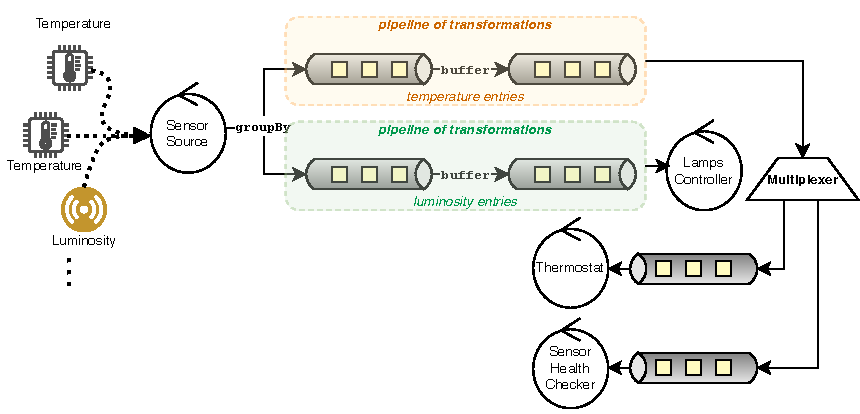
\includegraphics[width=0.8\textwidth]{./images/iot.pdf}
        \end{figure}
    \end{example}
\end{frame}

%--------------------------------------------------------------------------------

\begin{frame}
    \begin{itemize}
        \item Tasks provide a way to schedule them, possibly repeating them
        \begin{itemize}
            \item Different strategies: \texttt{Every}, \texttt{ExponentialBackoff}, \texttt{FibonacciBackoff}, \texttt{RepeatUntilFailure}, \texttt{RepeatUntilSuccess}.
        \end{itemize}
        \item To avoid the work-stealing behavior of channel consumers, a \texttt{ChannelMultiplexer} can be used. It is essentially a container of Readable and Sendable channels, which can be added and removed at runtime.
        \begin{itemize}
            \item Order is guaranteed only per producer;
            \item Typically, the consumer creates a channel and adds it to the multiplexer, then starts reading from it, possibly using a scheduled task.
        \end{itemize}
    \end{itemize}
\end{frame}

%--------------------------------------------------------------------------------

\begin{frame}
    \lstinputlisting[language=scala]{listings/Boundary.scala}
\end{frame}

%--------------------------------------------------------------------------------

\begin{frame}
    \lstinputlisting[language=scala]{listings/Iot.scala}
\end{frame}

%--------------------------------------------------------------------------------

\begin{frame}
    An example of a stateful Consumer:
    \lstinputlisting[language=scala]{listings/Consumer.scala}
    \footnotesize
    (see \texttt{smart-hub} module)
\end{frame}

%--------------------------------------------------------------------------------

\begin{frame}
    \lstinputlisting[language=scala]{listings/Controller.scala}
\end{frame}

%--------------------------------------------------------------------------------

\begin{frame}
    Since Scala \texttt{gears} currently doesn't provide any kind of transformation functions, few of them have been implemented (inspired by Rx):
    \begin{itemize}
        \item \texttt{map}
        \item \texttt{filter}
        \item \texttt{debounce}
        \item \texttt{groupBy}
        \item \texttt{buffer}
        \item \texttt{bufferWithin}
    \end{itemize}
    \footnotesize
    (see \texttt{PipelineTransformations.scala})
\end{frame}

%--------------------------------------------------------------------------------

\begin{frame}
    \lstinputlisting[language=scala]{listings/HubManager.scala}
\end{frame}

%--------------------------------------------------------------------------------

\begin{frame}
    \footnotesize
    To produce a testable version of this example, a simulated source of sensor data has been created, backed to a GUI, through which the user can simulate sensor behavior.
    \begin{figure}
        \centering
        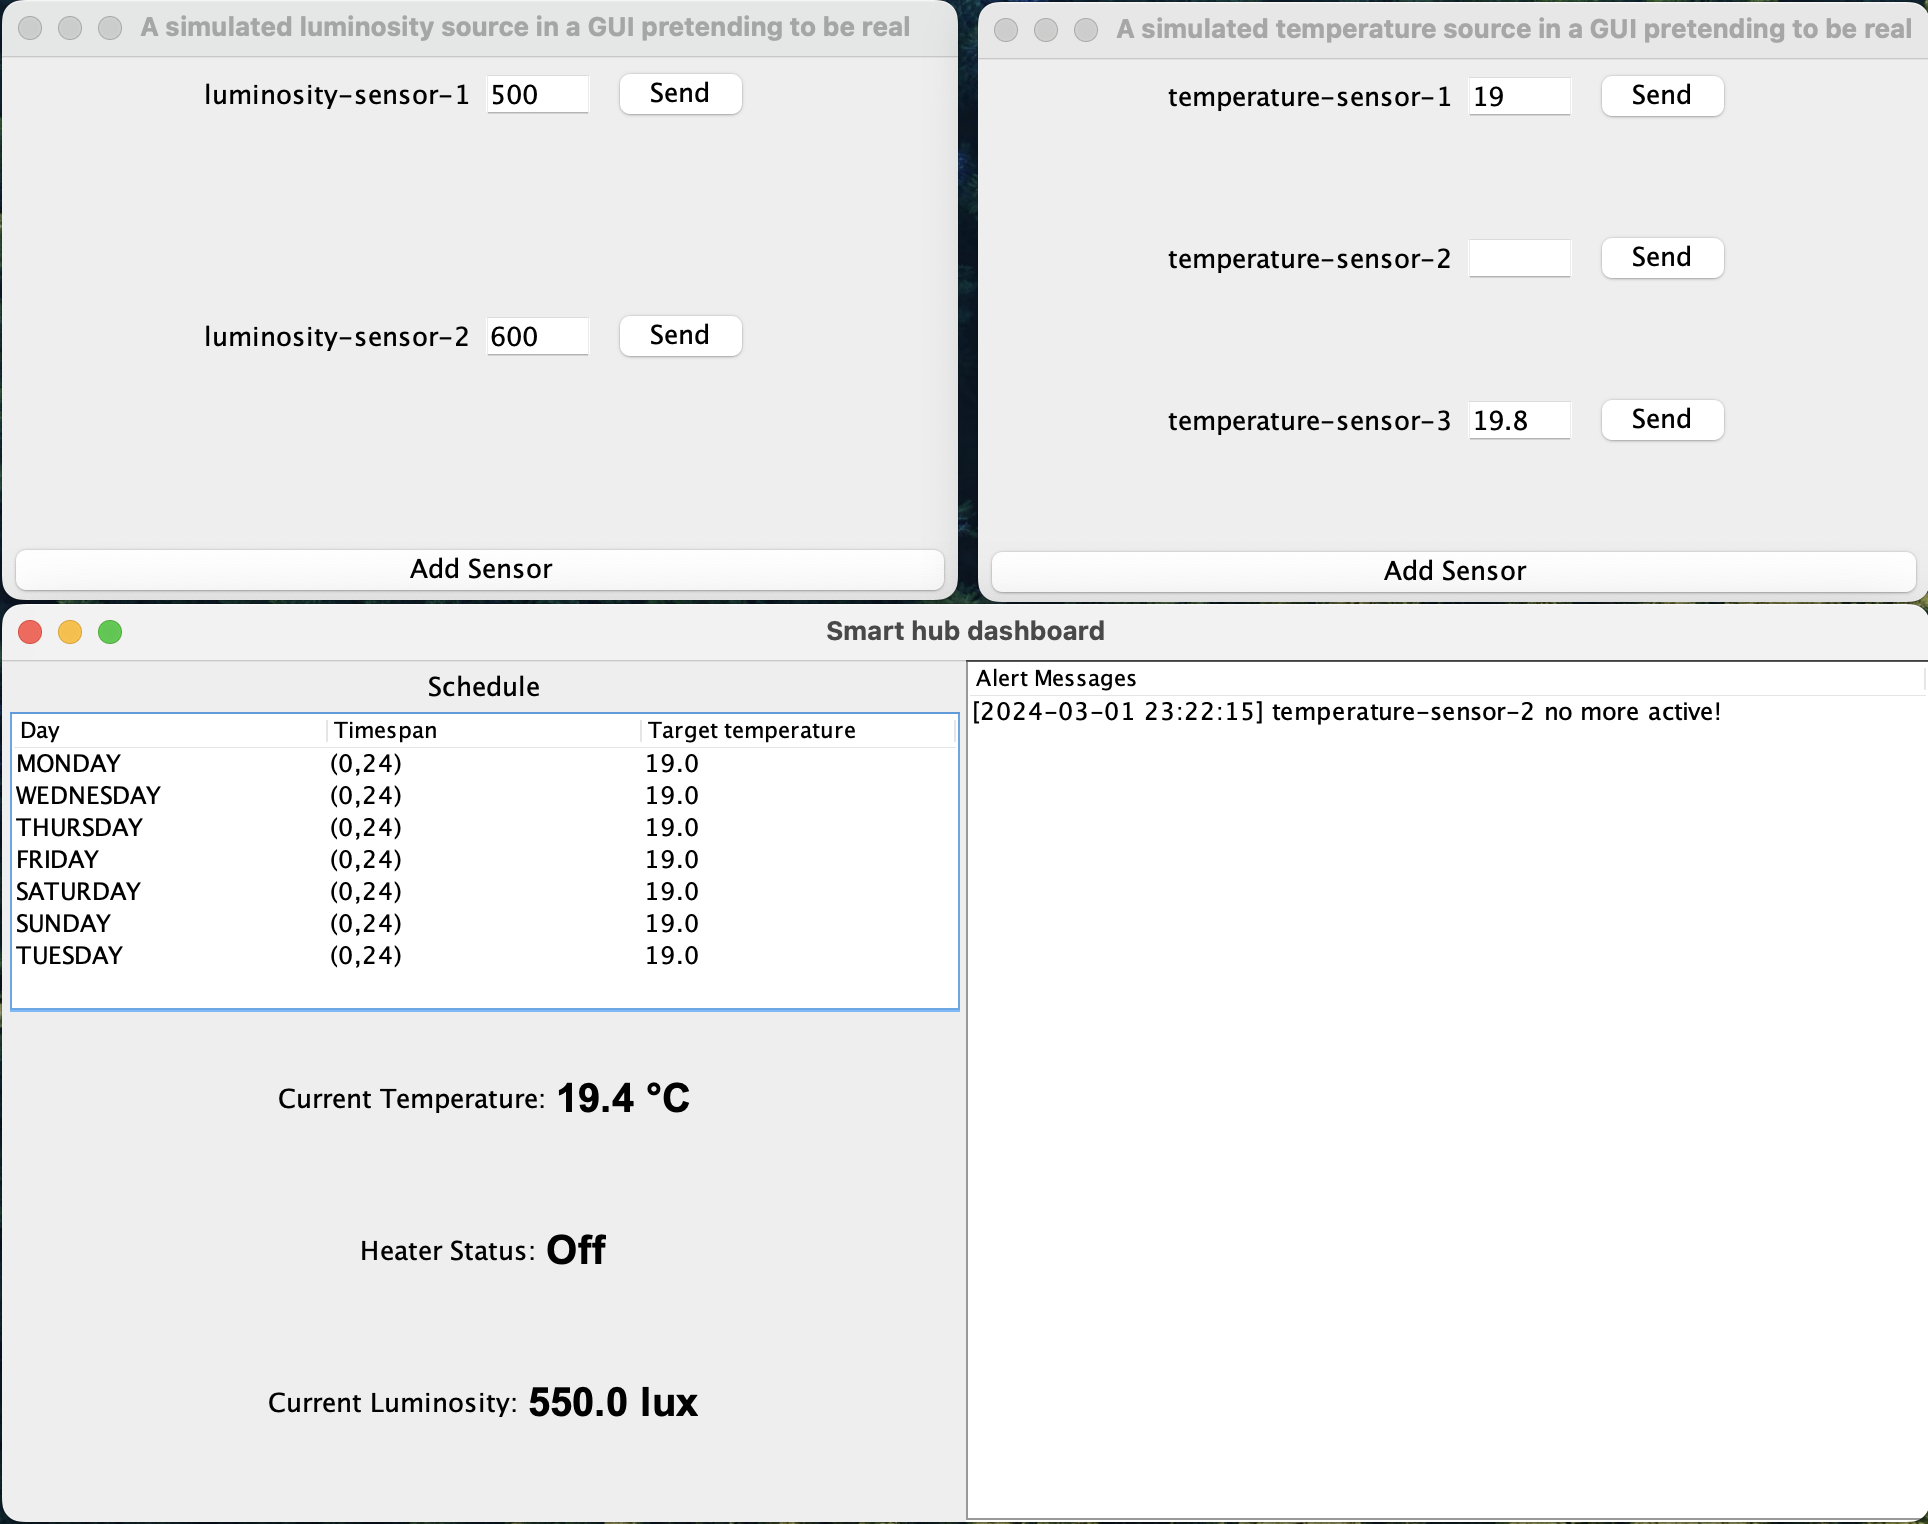
\includegraphics[width=0.6\textwidth]{./images/smart-hub.png}
    \end{figure}
\end{frame}

%--------------------------------------------------------------------------------

\begin{frame}{Conclusions}
    \begin{itemize}
        \item Direct style frameworks are arising as a natural and intuitive way to handle concurrency, leveraging an imperative-like programming style that is familiar to all developers.
        \item Scala gears, despite being a very young project, provides a good set of abstractions for asynchronous programming, although it cannot yet be considered a mature library ready to be used in a production environment:
        \begin{itemize}
            \item some design choices should be addressed (like closing a channel and the task scheduling)
            \item the library is still missing some important abstractions, like the proposed Flow for handling a cold stream of asynchronously computed values, and operators for functionally transforming channels
            \item  the project has been created for experimenting, thus performances have not been considered a priority so far
        \end{itemize}
    \end{itemize}
\end{frame}

%--------------------------------------------------------------------------------

\begin{frame}{References}
    % Beamer does not support BibTeX so references must be inserted manually
    \footnotesize{
        \begin{thebibliography}{99}
            \bibitem{capabilities} M. Odersky, A. Boruch-Gruszecki, E. Lee, J. Brachthäuser, O. Lhoták (2022)
            \newblock Scoped Capabilities for Polymorphic Effects
            \newblock \emph{\href{https://doi.org/10.48550/arXiv.2207.03402}{https://doi.org/10.48550/arXiv.2207.03402}}
            %------------------------------------------------
            \bibitem{can-throw} CanThrow Capabilities 
            \newblock Scala 3 nightly documentation
            \newblock \emph{\href{https://dotty.epfl.ch/docs/reference/experimental/canthrow.html}{https://dotty.epfl.ch/docs/reference/experimental/canthrow.html}}
            %------------------------------------------------
            \bibitem{scalar-gears} M. Odersky (2023)
            \newblock Direct Style Scala @ Scalar Conference 2023 
            \newblock \emph{\href{https://github.com/lampepfl/gears/blob/main/scalar-slides.pdf}{https://github.com/lampepfl/gears/blob/main/scalar-slides.pdf}}
            %------------------------------------------------
            \bibitem{gears} Scala \texttt{gears}
            \newblock Programming Methods Laboratory EPFL
            \newblock \emph{\href{https://github.com/lampepfl/gears}{https://github.com/lampepfl/gears}}
        \end{thebibliography}
    }
\end{frame}

%------------------------------------------------

\end{document}